% Options for packages loaded elsewhere
\PassOptionsToPackage{unicode}{hyperref}
\PassOptionsToPackage{hyphens}{url}
%
\documentclass[
  12pt,
]{article}
\usepackage{lmodern}
\usepackage{amssymb,amsmath}
\usepackage{ifxetex,ifluatex}
\ifnum 0\ifxetex 1\fi\ifluatex 1\fi=0 % if pdftex
  \usepackage[T1]{fontenc}
  \usepackage[utf8]{inputenc}
  \usepackage{textcomp} % provide euro and other symbols
\else % if luatex or xetex
  \usepackage{unicode-math}
  \defaultfontfeatures{Scale=MatchLowercase}
  \defaultfontfeatures[\rmfamily]{Ligatures=TeX,Scale=1}
  \setsansfont[]{Times New Roman}
\fi
% Use upquote if available, for straight quotes in verbatim environments
\IfFileExists{upquote.sty}{\usepackage{upquote}}{}
\IfFileExists{microtype.sty}{% use microtype if available
  \usepackage[]{microtype}
  \UseMicrotypeSet[protrusion]{basicmath} % disable protrusion for tt fonts
}{}
\makeatletter
\@ifundefined{KOMAClassName}{% if non-KOMA class
  \IfFileExists{parskip.sty}{%
    \usepackage{parskip}
  }{% else
    \setlength{\parindent}{0pt}
    \setlength{\parskip}{6pt plus 2pt minus 1pt}}
}{% if KOMA class
  \KOMAoptions{parskip=half}}
\makeatother
\usepackage{xcolor}
\IfFileExists{xurl.sty}{\usepackage{xurl}}{} % add URL line breaks if available
\IfFileExists{bookmark.sty}{\usepackage{bookmark}}{\usepackage{hyperref}}
\hypersetup{
  hidelinks,
  pdfcreator={LaTeX via pandoc}}
\urlstyle{same} % disable monospaced font for URLs
\usepackage[margin=1in]{geometry}
\usepackage{longtable,booktabs}
% Correct order of tables after \paragraph or \subparagraph
\usepackage{etoolbox}
\makeatletter
\patchcmd\longtable{\par}{\if@noskipsec\mbox{}\fi\par}{}{}
\makeatother
% Allow footnotes in longtable head/foot
\IfFileExists{footnotehyper.sty}{\usepackage{footnotehyper}}{\usepackage{footnote}}
\makesavenoteenv{longtable}
\usepackage{graphicx,grffile}
\makeatletter
\def\maxwidth{\ifdim\Gin@nat@width>\linewidth\linewidth\else\Gin@nat@width\fi}
\def\maxheight{\ifdim\Gin@nat@height>\textheight\textheight\else\Gin@nat@height\fi}
\makeatother
% Scale images if necessary, so that they will not overflow the page
% margins by default, and it is still possible to overwrite the defaults
% using explicit options in \includegraphics[width, height, ...]{}
\setkeys{Gin}{width=\maxwidth,height=\maxheight,keepaspectratio}
% Set default figure placement to htbp
\makeatletter
\def\fps@figure{htbp}
\makeatother
\setlength{\emergencystretch}{3em} % prevent overfull lines
\providecommand{\tightlist}{%
  \setlength{\itemsep}{0pt}\setlength{\parskip}{0pt}}
\setcounter{secnumdepth}{5}
\usepackage{booktabs}
\usepackage[]{natbib}
\bibliographystyle{apalike}

\title{Perceptions of Leaders}
\author{Casey Osorio-Duffoo}
\date{}

\begin{document}
\maketitle

{
\setcounter{tocdepth}{2}
\tableofcontents
}
\newpage

\hypertarget{abstract}{%
\section{Abstract}\label{abstract}}

This study examines the effect of active listening on perceptions of leaders. It is based on the knowledge that emotional intelligence is a fundamental component to good leadership and competent listening skills are central to demonstrating this form of intelligence. Research from multiple domains has shown that active listening leads to more positive perceptions, enhanced perspective-taking, and reductions in intergroup conflict. Because such outcomes are often associated with successful leaders, I hypothesized that leaders who demonstrate active listening would be perceived more favorably than leaders who do not. Participants were presented with two vignettes: one a professor and the other a business manager. The vignettes were created to show active listening, inactive listening, or information without interaction. Ratings were then completed on each leader. Preliminary data support the claim that leaders are perceived more favorably when they demonstrate active listening.

Keywords: active listening, emotional intelligence, leadership
\newpage

\hypertarget{perception-of-leaders}{%
\section{Perception of Leaders}\label{perception-of-leaders}}

~~~~~~Listening is a skill that everyone uses in their daily lives; it allows for interaction and communication with others. Listening is a skill which helps one person understand another. Listening is an important part to much a larger skill, which is emotional intelligence. Emotional intelligence ``organize a number of specific mental abilities having to do with identifying, understanding, managing and using emotions'' (Mayer, Salovey, \& Caruso, 2008). A good leader with high emotional intelligence should have excellent listening skills; therefore, being able to understand others and communicate effectively with others. Previous research has suggested that listening correlates with leaders' skills (Flynn, Valikoski, \& Grau, 2008; Kluger \& Zaidel, 2013), people who perceive leaders as good listeners increases employee commitment, self-awareness, and decrease intergroup conflict, and social anxiety (Bambacas, \& Patrickson, 2008; Bruneau, \& Saxe, 2012; Itzchakov, DeMarree, Kluge, \& Turjeman-Levi, 2018).

\emph{Emotional Intelligence and Leaders}

~~~~~~Emotional intelligence is a skill that leaders should have in any environment. Two questions about emotional intelligence are: what is emotional intelligence, and what are the effects of emotional intelligence?

~~~~~~Greenockle (2010) breaks down emotional intelligence into six different parts. First, self-awareness is being able to monitor and observes oneself (Greenockle, 2010). Leaders having self-awareness of their emotions and surrounding is crucial because it allows them to handle situations around them. Jassawalla, Truglia, \& Garvey observe leaders' self-awareness in cross-cultural situations was beneficial to have because leaders were able to differentiate between their culture and another's and adjusting to new cultural norms (2004). Self-awareness allows a leader to see what they are lacking and how they can go about being better, which would help in relationships. Second, self-management is being in control of one's own emotions, actions, and reactions, regardless of the situation (Greenockle, 2010). Jassawalla et al.~observe a similar component of emotional intelligence, which they called self-regulation (2004). Self-regulation is being open, managing uncertainties, and being flexible and patient in any situation (Jassawalla et al., 2004). Self-management and self-regulation are similar in that one have to manage their actions and feelings in any situation, which mean being flexible and patient will help in a conflict situation (Greenockle, 2010; Jassawalla et al., 2004). Third, self-motivation is maintaining optimism, confidence, and resilience in the face of setbacks and obstacles (Greenockle, 2010). Jassawalla et al.~observed that leaders that maintain self-motivation in the face of challenges were able to handle stress and find new ways to achieve assignment goals (2004). Fourth, communication skills are accurately conveying ideas, thoughts, feelings, emotions to others, and listening to what another is saying (Greenockle, 2010). Bambacas \& Patrickson asked Human Resources Manager were interpersonal communication skills they expected their managers to have (2008). Bambacas \& Patrickson found that sending messages and listening were the top two skills managers need to have (2008). This result shows that communicating with others effectively and efficiently and listening to what others say is essential in the real world. Fifth, interpersonal experience is being able to analyze a relationship and communicating that ``allows for effective exchange of information'' (Greenockle, 2010). In other words, one has to be aware and understanding of other's emotions. Côté explains that being able to see and to understand other emotions is important because it gives information about a person's attitude, goals, and intentions (2017). A leader needs to be able to see and understand the emotion of others to see what they strive for, and how they feel in a particular situation. Sixth, emotional mentoring is ``helping others help themselves'' (Greenockle, 2010). Emotional mentoring is keeping one's emotional perspective intact, not allowing someone's else emotion like anger to cause the same reaction in oneself (Greenockle, 2010). To be good at emotional mentoring as well as the other five components, one must be good at listening either to themselves or to others. Emotional intelligence is helpful in teams and groups of people. Emotional intelligence helps create proper communication and feedback between employees and managers. Abraham saw that emotional intelligence is linked to performance feedback (1999). Giving feedback or criticism allows for employees to learn about their current performance and how to improve their performance in the workplace (Abraham, 1999). Emotional intelligence helps with giving performance feedback because it allows the manager to place themselves in the employees' shoes and understand the employee's feelings (Abraham, 1999). In result, emotional intelligence allows the manager to pay attention to their words and tone that they used when giving employee feedback (Abraham, 1999).

~~~~~~Furthermore, providing feedback is another quality that manager needs in the workplace (Bambacas \& Patrickson, 2008). Providing proper feedback improves the employees' skills and performance (Abraham, 1999) and improves the organization overall (Bambacas \& Patrickson, 2008). Furthermore, leaders who have emotional intelligence would also be more satisfied with social support in the workplace (Schutte, \& Loi, 2014). Therefore, leaders would be more open to feedback and advice, which is an essential skill for leaders to have in the workplace (Bambacas \& Patrickson, 2008). Emotional intelligence can also help with organizational commitment. The organization wants its employees to be committed to the organization or company. Commitment meant companies wanted employees to have strong identification and involvement with the company (Abraham, 1999). Leaders with emotional intelligence will have the ability to manage their emotions in a stressful situation, and self-motivate themselves in front of obstacles (Greenockle, 2010); they will be turning all of negative feelings and energy into positive, which improves job satisfaction, and organization commitment (Abraham, 1999). Furthermore, emotionally intelligence leaders who create a supportive work environment for teams and groups will lead to stronger commitment to the team, and in turn, a stronger commitment to the organization (Abraham, 1999). Leaders who have emotional intelligence can positively impact the workplace in many ways. In results, these leaders with emotional intelligence achieve more positive workplace outcomes, and therefore, leaders are more effective and seen as more effective by subordinates and direct managers (Rosete \& Ciarrochi, 2005). Rosete \& Ciarrochi studied an ability based model of emotional intelligence and how it is positively associated with effective leadership, and they measured this prediction through a performance management system (2005). Rosete \& Ciarrochi looked at four dimensions of emotional intelligence which were: ``perceiving emotions accurately, using emotion to facilitate thought; understanding emotion, and managing emotions'' (2005). These four dimensions are similar to Geenockle's six competent of emotional intelligence (2010), and to other studies that observed emotional intelligence. Rosete \& Ciarrochi found that emotional intelligence is positively associated with effective leadership, and who is and who is not able to deal effectively with colleagues and staff (2005). Being able to get along with colleagues and staff is essential, mainly since problems and situation already occur in the workplace. People who are not able to get along with their colleagues and staff are adding more problems to the workplace.

~~~~~~Emotional intelligence can help with managing conflict in the workplace. There are always going to be situations and conflicts that arise in the workplace, and a manager with emotional intelligence should be able to handle it. In cases like this, a manager with emotional intelligence will be able to understand the emotions and feelings in a situation and come up with a modify the situation by taking a break (Côté, 2017), so people will have a moment to relax and calm down from the situation. On the other hand, managers must also be to motivates and inspire themselves and their employees, not just calm employee down when angry or stress. Magnano, Craparo, \& Paolillo look at resilience and emotional intelligence in achievement motivation (2016). Magnano et al.~hypothesis emotional intelligence will be positively related to achievement motivation and resilience, while resilience mediates the relationship between emotional intelligence and achievement motivation (2016). Magnano et al.~found that all three of their hypothesis were supported (2016). The implications were that emotional intelligence plays in role in people's resilience and their growth (Magnano et al., 2016). Also, resilient people are described as emotional intelligence and use their positive emotion to help against difficult challenges (Magnano et al., 2016). Lastly, a person who accurately perceives, access, and regulates their emotions can deal better in a stressful work environment, and achieve organization goals (Magnano et al., 2016). Emotional intelligence is a need for resilience, and resilience is one way where emotional intelligence can lead to better motivation at work (Magnano et al., 2016). The results from Magnano et al.~(2016) shows why leaders need to have emotional intelligence since they would be able to deal in a stressful work environment, be properly motivated, and they should be able to help others do the same. One important competent of emotional intelligence, which further intensifies providing and receiving feedback, organization commitment, and create a safe and supportive environment for others is through listening.

\emph{Impact of Leaders' Listening}

~~~~~~Leaders must be able to listen to others, but listening is not merely hearing another person. Leaders must be able to actively listen to others, which is involves asking a question, supporting another, be cooperative, and give feedback (Zenger \& Folkman, 2016). Asking questions lets the person know that they are being heard (Zenger \& Folkman, 2016). People feeling that they are being heard has shown to decrease conflict between groups (Bruneau \& Saxe, 2012; Gutenbrunner \& Wagner, 2016). Bruneau \& Saxe study looks at dialogue-based intervention could improve inter-group attitudes, in groups with conflict (2012). Participants were either perspective taking or perspective giving in the experiment (Bruneau \& Saxe, 2012). Bruneau \& Saxe did this by creating the feeling of being heard, where the responder wrote a summary of the sender's statement, in their own words, without expressing their thoughts, beliefs, or suggestion (2012). The implication from the results was that in perspective-taking condition, people empowered attitudes to improve towards disempowered people, and in the perspective-giving condition, the attitudes of disempowered improved toward empowered (Bruneau \& Saxe, 2012). This implication can be applied to leaders in that if leaders make others feel heard, it would improve employees' attitudes, and decrease conflict between leaders and employees. Gutenbrunner \& Wagner also look at perspective, taking decreasing conflict between people (2016). Gutenbrunner \& Wagner looked at different types of perspective, taking techniques to decrease conflict, which controlled dialogue and role reversal (2016). Controlled dialogue is to repeat what the other person says first, and then respond (Gutenbrunner \& Wagner, 2016). The controlled dialogue was similar to Bruneau's \& Saxe's (2016) study in creating the feeling of being heard. In both Bruneau et al.~(2012), and Gutenbrunner et al.~(2016), their simple methods of having participant repeat what the other is saying either verbally or written created a feeling of being heard in the other participant. Furthermore, the results showed that the feeling of being heard did improve attitude change towards an opposing group (Bruneau \& Saxe, 2012; Gutenbrunner \& Wagner, 2016). The results show that people who make one person or even a group of people feel heard will tend to decrease conflict between that one person or group people. Leaders need to be able to do the same for those around them, especially in the workplace.

~~~~~~Leaders who listen, support, and build confidence in others, and they are cooperative in conversation (Zenger \& Folkman, 2016). Since, listening involves creating a safe and supportive environment, where people can talk about their thoughts and opinions (Zenger \& Folkman, 2016) and therefore, increasing one's attitude clarity, self-awareness, and reduces social anxiety (Itzchakov, DeMarree, Kluge, \& Turjeman-Levi, 2018). People being able to talk out their ideas and opinions helps them realize their position in a situation, and they start to be less afraid of being negatively judged by others if they knew someone was listening to them (Itzchakov et al., 2018). Furthermore, leaders who listen to challenges others assumptions because then it allows for one to thinks more about their assumptions, which again helps in attitude clarity and self-awareness.

~~~~~~Listening also involves giving suggestions or feedback in order to help another person (Zenger \& Folkman, 2016). Giving proper feedback or advice is difficult, since managers may feel uncomfortable criticizing their employees (Abraham, 1999), or employees being stressed and defensive about feed will downplay the importance of the person providing the feedback (Itzchakov \& Kluger, 2018). Furthermore, giving proper feedback is hard, when neither the manager or employee sees the other perspective. If the manager does not see the employee's feedback of how it feels, and the employee does not see why the manager has to give feedback, then giving and receiving feedback would be harder for both sides. However, listening can significantly enhance the interpersonal relationship in business, and proper feedback is crucial for both managers and employees (Longweni \& Kroon, 2018). In one experiment, the participant was randomly assigned to a listening group: good, moderate, and poor (Itzchakov \& Kluger, 2018). Participant in the excellent listening condition talks about their strengths and weaknesses (Itzchakov \& Kluger, 2018). Participant in the poor or distracted listening condition talk about their strengths and barely mention their weaknesses (Itzchakov \& Kluger, 2018). The result shows that listening allows for an employee more aware of their weakness and strengths and reflects on them in a non-defensive manner (Itzchakov \& Kluger, 2018). Employees who are aware of their strengths and weakness and improves themselves will only help the company, and one way for this to happen is to have a leader who listens. Also, employees have different skills, abilities, and levels of education, which can play a factor in how they perceive the effectiveness of their manager. Longweni \& Kroon observed how employees with different education backgrounds perceive the effectiveness of their managers' listening and feedback skills, and the managers' ability to deal with interference during listening and feedback (2018). Longweni \& Kroon used a survey to conduct the experiment (2018). Longweni \& Kroon found that there was a significant difference on how subordinates with different education backgrounds perceive their manager's listening and feedback skills, and their manager's ability to deal with interference during listening and feedback (2018). Their results implied that effective communication is essential in promoting and sustaining a business (Longweni \& Kroon, 2018).

~~~~~~Listening is a component of emotional intelligence (Greenockle, 2010) can also increase organizational commitment (Bambacas \& Patrickson, 2008). A leader who communicates clearly and are consistent with sending message increase organization commitment (Bambacas \& Patrickson, 2008). Specifically, in order to enhance commitment, delivering message need to focus on the individual receiving the message, while making the message coherent, engaging, and interpreted correctly (Bambacas \& Patrickson, 2008). Therefore, leaders have to be aware to the message they send to their employees since the interaction is shaped from external factors like culture, economy, and competitiveness, as well as individual factors like listening habits, motivations, and perceptions (Bambacas \& Patrickson, 2008). A leader needs to pay attention to everyone as a whole and individually in order to be effective in communication, which will help create stronger organizational commitment.

~~~~~~Active listening is an essential competent in emotional intelligence since people can perceive leaders who actively listen. Leaders who actively listen to other can enhance organization commitment, self-awareness, give proper feedback, decrease conflict, and social anxiety (Bambacas \& Patrickson, 2008; Bruneau \& Saxe, 2012; Itzchakov et al., 2018; Longweni \& Kroon, 2018). Therefore, the first hypothesize is that leaders who exhibit listening, and communications skills will be perceived as more competent than leaders who do not. Since, leaders who possess active listening skills are seen as more helpful, attentive, and cooperative with others.

~~~~~~Furthermore, the second hypothesize is that students would rate professors who listen to be more competent than managers who listen. In this current research, students will be presented with two different types of leaders (manager, professor), and assesses participants' perceptions of these leaders based on whether they demonstrate listening skills. Since, students have more contact and bonding with a professor, rather than a manager; students would have more of a connection with the professor and view the professor as a more competent leader when displaying active listening skills.

\newpage

\hypertarget{methods}{%
\section{Methods}\label{methods}}

\emph{Participants}

~~~~~~Data was collected from Seton Hall Undergraduate students, who were recruited through Seton Hall University SONA system. Participants received extra credit in their class for participation. All participants were asked to bring their laptops in order to complete the experiment. Our sample size consisted of 86 students. Sixty-six of the participants were female, and the other 20 were male. Students' academic year broke down as follow: forty-eight Freshmen, twenty-six Sophomores, eleven Juniors, and one Senior. Also, the average participants' age was approximately 19.1 (SD=1.09). Participants' race consists of 37 White, 22 Hispanic/Latino, 18 Asian, and 7 Black or African American. Participants were also asked if they worked or not, and 50 participants had a job, and 36 participants did not have a job. More specifically, 3 participants had a full-time job, 32 participants had part-time jobs, and 15 participants work intermittently.

\emph{Materials}

~~~~~There were six vignettes created for this study. The vignettes were about two different leaders (manager, professor). The vignettes portrayed demonstrated the leader's listening skills (Active Listening, Gives out Orders, Control Condition) in a workplace or a classroom. Participants read two vignettes about one type of leader's listening skills on both the manager and professor. In the Active Listening condition, Professor N takes the time to listen to the students' concerns, ask for feedback, and solve any problems that the students addressed with the class. In the Giving out Order or Inactive Listening condition, Professor N explains the course to the students, and ask for feedback, when the student express their concerns. The professor does not acknowledge their concerns and continues by explaining the course. In the control condition, Professor N does not show any listening skills and does not engage with the students for feedback, and Professor N explains what point after the other. Participants were randomly assigned to one of three conditions and randomly assigned to the order in which leader they read about first the manager or professor.

\emph{Perception Ratings}

~~~~~~Participants' perceptions concerning the leaders' listening skills were obtained using a survey. The survey commenced with a statement asking the participant to rate the items. The survey was a 7-point Likert scale, which measured the leader's listening skills, communication skills, and emotional intelligence. The endpoints of the scales were labeled (1= Strongly Disagree with the statement, and 7= Strongly Agree with the statement).

\emph{Procedure}

~~~~~~Participants were randomly assigned to a condition using a random number generator. The participant received an email with a link to the experiment. Once participants open the experiment, they read the instructions for the experiment and started reading the first vignette. After the first vignette, participants rated their perceptions on the first leader on the 1-7 scales, and the participant was asked if the leader is good, open to change, communicate well, etc. Next, the participants read the second vignette on the second leader. The participants rated their perception again on a 1-7 scale using similar statements as on the previous leader. After the participants finish the experiment, they were debriefed about the experiment.

\hypertarget{results}{%
\section{Results}\label{results}}

~~~~~~The Statistical Package for Social Sciences (SPSS) and Jamovi were used in this study to analyze the data. Exploratory factor analyses showed two factors: one for the professor vignette and one for the manager. Then, a composite score of the items for the professor and the manager. The composite score of the professor consist of factors that load highly, which were: 1) a good professor, 2) would take a class with this professor, 3) a skilled leader, 4) an effective leader, 5) high emotional intelligence, 6) a weak leader, 7) cares little about students, 8) open to feedback, 9) not open to change, 10) communicates poorly, and 11) good at listening. The composite score of the manager consists of factors that load highly, which were: 1) a good manager, 2) would work for this manager, 3) a skilled leader, 4) an effective leader, 5) high emotional intelligence, 6) a weak leader, 10) communicate poorly, and 11) good at listening (Table 1, Appendix A). Also, for any negative statements like ``weak leader'' or ``communicate poorly,'' the scores were reversed. Therefore, instead of being low ratings like 1 or 2, the rating will be 7 or 6, and then, with those scores, the composite score for both the manager and professor were created.

~~~~~~A Repeated Measures ANOVA was conducted using the two composite scores from the factor loadings. There was a significant effect for type of leader: F (1, 83)= 4.945, p\textless.029, which meant participants were favoring one type of leader over another. The active professor was rated significantly higher than both control and inactive professor. The average mean score of the active professor was (M=6.01), while the control professor was (M=5.42) and the inactive professor was (M=4.65) (Table 2). The active manager was rated significantly higher than both control and inactive manager. The average mean score of the active manager was (M=5.92), while the control manager was (M=5.23) and the inactive manager was (M=4.06) (Table 2). The results support our first hypothesis. There was no interaction between leaders and conditions. The ANOVA further revealed a significant effect among all three conditions.

~~~~~~A MANOVA was conducted to follow up on the prior testing that looks at the type of leader. The MANOVA revealed a significant effect between

conditions for the professor and manager: F (2, 83)= 42.055, p\textless.000. A post-hoc test shows the difference between each condition. The professor in the active versus control conditions (MD=.58), active versus inactive conditions (MD=1.36), and control versus inactive conditions (MD=.77) (Table 3). The manager in the active versus control conditions (MD=.68), active versus inactive conditions (MD=1.85), and control versus inactive conditions (MD=1.17) (Table 3). The result supports our second hypothesis.

\begin{verbatim}
##  Response 1 :
##                              Df Sum Sq Mean Sq F value    Pr(>F)    
## Data$ConCond                  1  0.070  0.0701  0.0898    0.7652    
## Data$ListenCond               2 26.992 13.4960 17.3083 5.672e-07 ***
## Data$ConCond:Data$ListenCond  2  0.633  0.3166  0.4060    0.6677    
## Residuals                    80 62.379  0.7797                      
## ---
## Signif. codes:  0 '***' 0.001 '**' 0.01 '*' 0.05 '.' 0.1 ' ' 1
## 
##  Response 2 :
##                              Df Sum Sq Mean Sq F value    Pr(>F)    
## Data$ConCond                  1  0.291  0.2907  0.4208    0.5184    
## Data$ListenCond               2 59.382 29.6910 42.9830 2.103e-13 ***
## Data$ConCond:Data$ListenCond  2  1.535  0.7676  1.1113    0.3342    
## Residuals                    80 55.261  0.6908                      
## ---
## Signif. codes:  0 '***' 0.001 '**' 0.01 '*' 0.05 '.' 0.1 ' ' 1
\end{verbatim}

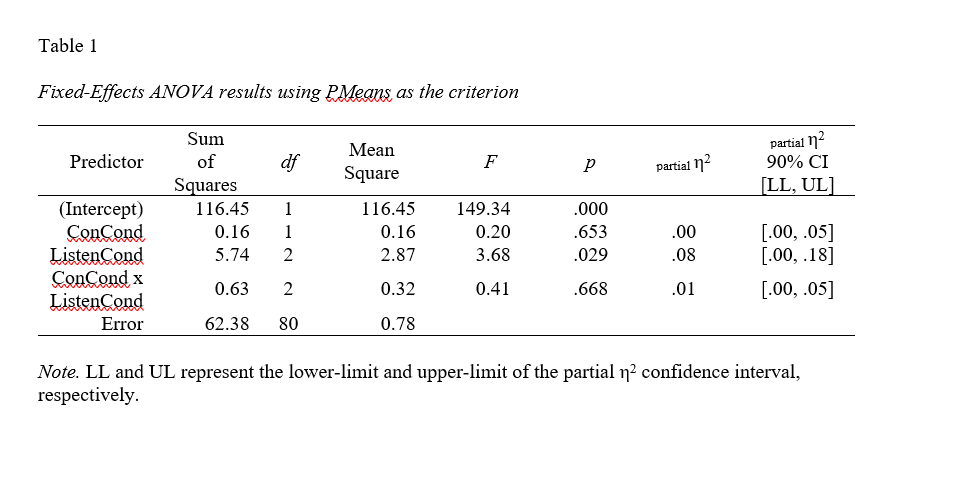
\includegraphics[width=13.46in]{Files/Table 1}
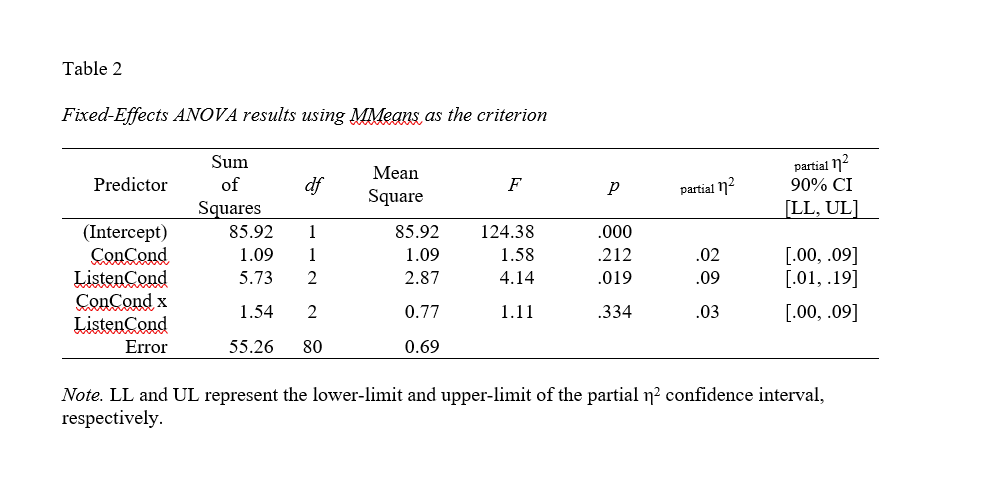
\includegraphics[width=13.78in]{Files/Table 2}

\hypertarget{discussion}{%
\section{Discussion}\label{discussion}}

We have finished a nice book.

  \bibliography{book.bib,packages.bib}

\end{document}
